%!TEX TS-program = xelatex
%!TEX encoding = UTF-8 Unicode
% -*- coding: UTF-8; -*-
% vim: set fenc=utf-8
%
% =============================================================
%  地质学学位论文示例：东昆仑造山带花岗岩锆石 U-Pb 年代学
%
%  这个文件的用途：模板功能演示 + 写作格式参考。
%   · 正文文字与数据均为示例，请替换为你自己的内容；
%   · 表格采用三线表（booktabs），横向大图采用 pdflscape；
%   · 编译：xelatex -shell-escape sample.tex（或 build.bat sample）
%
%  格式一律以中国地质大学（武汉）研究生院最新版
%  《研究生学位论文写作规范》为准，见 README 的免责声明。
% =============================================================

\documentclass[master]{cugthesis}
% 学位类型：doctor / master / masterprofulltime / masterpronofulltime

\usepackage{booktabs}       % 三线表（规范 2.5.2 建议采用）
\usepackage{pdflscape}      % 横向页面，放大图或宽表
\usepackage{multirow}

% ---------------- 基本信息 ----------------
\cugthesistitle{东昆仑造山带晚古生代花岗岩锆石 U-Pb 年代学与地球化学特征}%
    {Zircon U-Pb Geochronology and Geochemistry of Late Paleozoic Granitoids in the East Kunlun Orogenic Belt}
\cugthesisauthor{张三}{Zhang San}
\studentid{1202611347}
\cugthesismajor{地质学}{Geology}
\cugthesisteacher{某某某\quad 教授}{Prof.\ XXX}
\educatingunit{地球科学学院}
\cugthesisdate{2026}{6}

% ---------------- 封面字段（规范 1.1 / 附件 12）----------------
\cugclassnumber{P588}        % 分类号，查《中国图书馆分类法》
\cugsecretlevel{公开}        % 密级

% ---------------- 摘要 ----------------
\cugabstract{
    东昆仑造山带位于青藏高原北缘，是研究古特提斯洋俯冲消减与增生造山过程的关键地区。
    本文对造山带中段出露的晚古生代花岗质岩体开展了系统的岩相学、锆石 LA-ICP-MS
    U-Pb 定年与全岩地球化学研究。锆石 U-Pb 测年获得 $1851\pm17$ Ma 的谐和年龄，
    指示岩体侵位于中元古代晚期。岩石组合以花岗闪长岩和二长花岗岩为主，
    属高钾钙碱性准铝质—弱过铝质系列。岩石富集大离子亲石元素（Rb、Ba、Th、U），
    亏损高场强元素（Nb、Ta、Ti），稀土配分曲线呈右倾型并具中等负 Eu 异常，
    具有典型的俯冲带岩浆岩地球化学属性。综合区域地质资料认为，
    该期岩浆活动与古特提斯洋向北俯冲引起的幔源岩浆底侵及地壳重熔有关，
    为东昆仑地区晚古生代增生造山过程提供了新的年代学约束。
}{The East Kunlun Orogenic Belt, located on the northern margin of the
Qinghai--Tibet Plateau, is a key area for understanding the subduction and
accretionary processes of the Paleo-Tethys Ocean. In this study, zircon
LA-ICP-MS U-Pb dating and whole-rock geochemistry were carried out on Late
Paleozoic granitoids exposed in the central segment of the belt. Zircon U-Pb
analyses yield a concordia age of $1851\pm17$ Ma, indicating emplacement during
the late Mesoproterozoic. The rocks are mainly granodiorite and monzogranite,
belonging to the high-K calc-alkaline, metaluminous to weakly peraluminous
series. They are enriched in large ion lithophile elements (Rb, Ba, Th, U) and
depleted in high field strength elements (Nb, Ta, Ti), with right-leaning REE
patterns and moderate negative Eu anomalies, characteristic of arc-related
magmatism. Combined with regional geological data, this magmatism is
interpreted to be related to mantle upwelling and crustal anatexis induced by
northward subduction of the Paleo-Tethys Ocean.}

\cugkeywords{东昆仑造山带; 锆石 U-Pb 年代学; 花岗岩; 岩石成因; 古特提斯}%
    {East Kunlun Orogenic Belt; Zircon U-Pb geochronology; Granitoid; Petrogenesis; Paleo-Tethys}

% ---------------- 答辩委员会名单（规范 1.7 / 附件 7）----------------
\cugcommitteemember{主席}{某某某}{教授}{中国地质大学（武汉）}
\cugcommitteemember{委员}{某某某}{教授}{中国地质大学（武汉）}
\cugcommitteemember{委员}{某某某}{研究院}{中国地质科学院}
\cugcommitteemember{委员}{某某某}{副教授}{中国地质大学（武汉）}
\cugcommitteemember{秘书}{某某某}{讲师}{中国地质大学（武汉）}

\begin{document}

\makefrontpages

% =============================================================
\chapter{绪论}

\section{研究背景与意义}

东昆仑造山带地处青藏高原北缘、中央造山带西段，是原特提斯与古特提斯两期
洋盆俯冲消减、弧陆碰撞及陆内叠覆的复合造山带。
该区广泛出露古生代—中生代侵入岩，记录了原特提斯洋与古特提斯洋的
俯冲极性、时限及深部物质循环过程，长期是研究增生型造山作用的天然实验室。

花岗质岩石是大陆地壳的主要组成，其成因与就位机制对理解壳幔相互作用、
地壳生长与再造具有关键意义\citep{wu2007}。由于花岗岩对构造背景的响应
存在多解性，单靠地球化学判别往往不足以约束其形成环境，
必须与精细的年代学格架、区域地质以及同位素资料相互印证。
因此，获取高质量的中酸性侵入体年龄数据，是重建造山带演化序列的基础工作。

\section{研究现状}

\subsection{东昆仑造山带的岩浆期次}

前人研究将东昆仑地区的岩浆活动划分为若干个阶段，其中晚古生代—
早中生代被认为是古特提斯洋演化最为活跃的时期。
然而，由于测年方法与测试精度的差异，不同学者对同一岩体获得的年龄
跨度较大，部分岩体的时代归属仍存在争议。

\subsection{锆石 U-Pb 定年方法}

锆石因具有高的 U 含量、低的普通 Pb 含量和极强的抗改造能力，
是目前最可靠的 U-Pb 定年矿物。激光剥蚀电感耦合等离子体质谱
（LA-ICP-MS）技术在保证较高空间分辨率的同时，兼顾了分析效率，
已成为区域岩浆事件厘定的常规手段\citep{paton2011}。

锆石 U-Pb 体系的年龄由衰变方程给出：
\begin{equation}
    t=\frac{1}{\lambda_{238}}\ln\left(1+\frac{{}^{206}\mathrm{Pb}^{*}}{{}^{238}\mathrm{U}}\right)
    \label{eq:age}
\end{equation}
式中 $\lambda_{238}$ 为 ${}^{238}\mathrm{U}$ 的衰变常数，取值
$1.55125\times10^{-10}\,\mathrm{a}^{-1}$；${}^{206}\mathrm{Pb}^{*}$
为放射成因铅。当分析点同时满足谐和条件时，可用式 \eqref{eq:age} 直接计算
其 ${}^{206}\mathrm{Pb}/{}^{238}\mathrm{U}$ 年龄。

\section{研究内容与技术路线}

本文以东昆仑造山带中段出露的花岗质岩体为研究对象，开展以下工作：
（1）野外地质调查与样品采集；（2）岩相学观察；
（3）锆石 LA-ICP-MS U-Pb 定年；（4）全岩主量与微量元素地球化学分析；
（5）结合区域资料探讨岩石成因与构造意义。

% =============================================================
\chapter{区域地质概况}

\section{大地构造位置}

研究区位于东昆仑造山带中段，北以昆中断裂为界与昆北地体相邻，
南以昆南断裂与巴颜喀拉地体相接。区内主要出露古元古代—中元古代
变质基底、古生代火山—沉积岩系以及大量中酸性侵入岩体。

\section{地层与岩浆岩}

区内元古宇主要为片麻岩、片岩及大理岩组合，经历了角闪岩相—
绿片岩相变质作用。古生界以浅海相碳酸盐岩与碎屑岩为主。
侵入岩以花岗闪长岩、二长花岗岩为主，多呈岩基或岩株状产出，
与围岩呈侵入接触关系，局部见暗色微粒包体。

研究区构造格架与采样位置如图 \ref{fig:region} 所示。

% ---------- 横向页面（大图或宽表用）----------
% 用 pdflscape 的 landscape 环境，页面在 PDF 里会旋转 90°。
% 两点注意：
%   1. 横向页的页眉文字会被旋转到可视范围之外，故用 cuglandscape 页样式
%      「只印外侧页码、不印页眉文字」（该样式由模板提供）。
%      若学院要求横向页也带页眉，把这一行删掉再自行调整。
%   2. 用 center + \captionof 而不是 figure 浮动体，这样图片能在
%      横向页面里垂直居中，不会缩在页顶。
\begin{landscape}
\thispagestyle{cuglandscape}
\begin{center}
    \vspace*{\fill}
    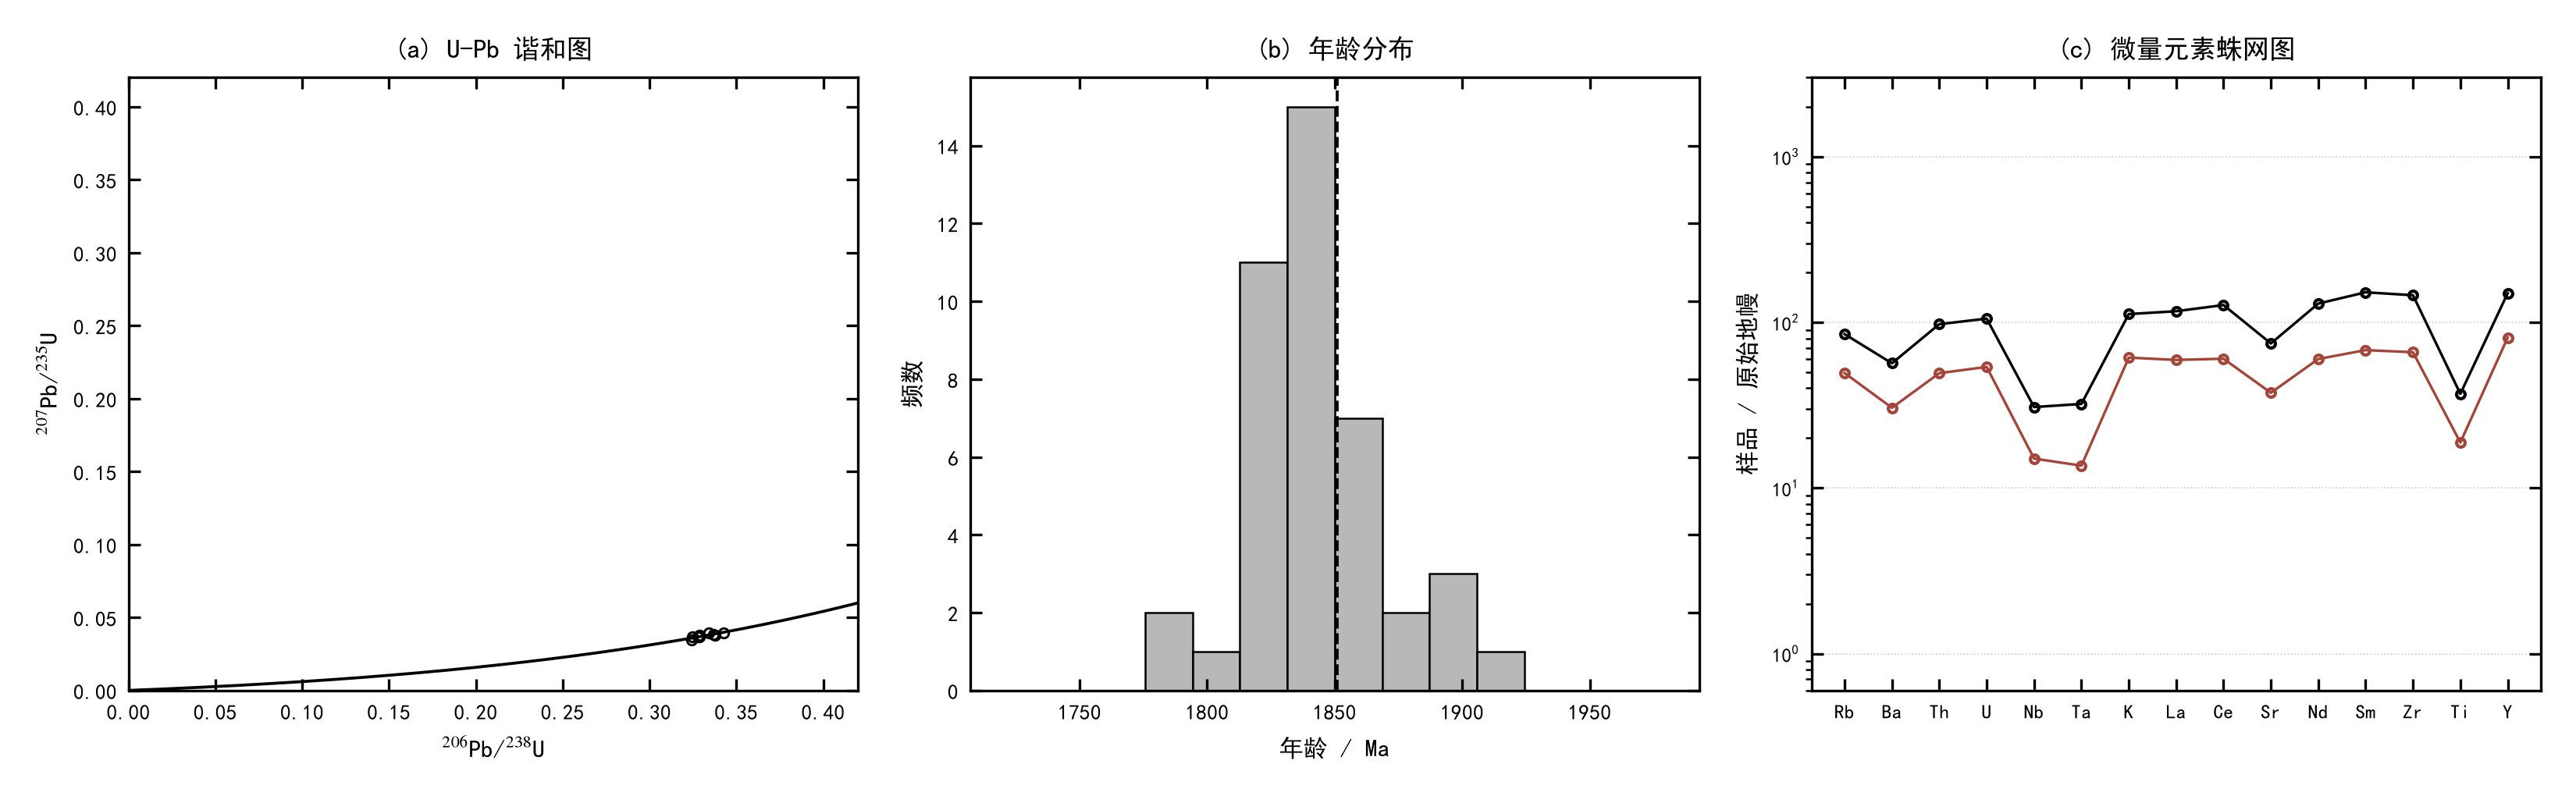
\includegraphics[width=.94\linewidth]{figs/fig_wide_summary.png}
    \vspace{1.2em}

    \captionof{figure}{东昆仑造山带中段花岗岩综合图解。（a）锆石 U-Pb 谐和图；
        （b）锆石 $^{206}$Pb/$^{238}$U 年龄分布直方图；
        （c）微量元素原始地幔标准化蛛网图}
    \label{fig:region}
    \vspace*{\fill}
\end{center}
\end{landscape}

% =============================================================
\chapter{样品与分析方法}

\section{样品采集与岩相学}

本次研究共采集新鲜无蚀变的花岗质岩石样品 12 件，采样位置见图 \ref{fig:region}。
样品呈灰白色—浅肉红色，中粒似斑状结构，块状构造。斑晶以斜长石、
钾长石为主，粒径 $2\sim5\,\mathrm{mm}$；基质由石英、斜长石、
角闪石及少量黑云母组成。副矿物见锆石、磷灰石、榍石及磁铁矿。

\section{锆石 U-Pb 定年}

\subsection{样品制备}

将岩石样品粉碎至 $60\sim80$ 目，经常规重选与电磁选分离出锆石。
在双目镜下挑选晶形完好、无包裹体与裂纹的锆石颗粒制片，
抛光后进行阴极发光（CL）成像，据此选定分析点位。

\subsection{LA-ICP-MS 分析条件}

锆石 U-Pb 同位素分析在配备 193 nm ArF 准分子激光的
电感耦合等离子体质谱仪上完成。激光束斑直径 $32\,\mu\mathrm{m}$，
剥蚀频率 $6\,\mathrm{Hz}$，能量密度约 $6\,\mathrm{J/cm^2}$。
以 NIST SRM 610 为外标、$^{29}\mathrm{Si}$ 为内标进行元素分馏校正，
采用标准锆石 91500 与 Plešovice 监控数据质量。
仪器工作参数见表 \ref{tab:condition}。

\begin{table}[htbp]
    \centering
    \caption{LA-ICP-MS 仪器工作参数}
    \label{tab:condition}
    \begin{tabular}{lll}
        \toprule
        项目 & 参数 & 备注 \\
        \midrule
        激光器 & 193 nm ArF 准分子 & \\
        束斑直径 & $32\,\mu\mathrm{m}$ & 可调 $16\sim44\,\mu\mathrm{m}$ \\
        剥蚀频率 & $6\,\mathrm{Hz}$ & \\
        能量密度 & $\sim 6\,\mathrm{J/cm^2}$ & \\
        载气 & He（$0.6\,\mathrm{L/min}$） & \\
        外标 & NIST SRM 610 & 元素含量校正 \\
        监控标样 & 91500、Plešovice & 年龄监控 \\
        \bottomrule
    \end{tabular}
\end{table}

\section{全岩地球化学分析}

主量元素采用 X 射线荧光光谱法（XRF）测定，分析精度优于 2\%；
微量元素与稀土元素采用电感耦合等离子体质谱法（ICP-MS）测定，
对多数元素的相对标准偏差优于 5\%。

% =============================================================
\chapter{分析结果}

\section{锆石 U-Pb 年龄}

锆石颗粒多呈无色透明—浅黄色，自形柱状，长宽比 $2{:}1\sim4{:}1$，
内部发育典型岩浆振荡环带。分析结果见表 \ref{tab:zircon}。

\begin{table}[htbp]
    \centering
    \caption{锆石 LA-ICP-MS U-Pb 同位素分析结果}
    \label{tab:zircon}
    \small
    \begin{tabular}{ccccccc}
        \toprule
        点号 & Th/U & $^{207}$Pb/$^{235}$U & $1\sigma$ & $^{206}$Pb/$^{238}$U
             & $1\sigma$ & 年龄/Ma \\
        \midrule
        01 & 0.62 & 4.812 & 0.061 & 0.3241 & 0.0038 & 1810 \\
        02 & 0.55 & 4.937 & 0.058 & 0.3308 & 0.0035 & 1843 \\
        03 & 0.71 & 5.021 & 0.066 & 0.3295 & 0.0041 & 1836 \\
        04 & 0.48 & 4.876 & 0.059 & 0.3262 & 0.0037 & 1820 \\
        05 & 0.66 & 5.104 & 0.063 & 0.3336 & 0.0039 & 1856 \\
        06 & 0.59 & 4.998 & 0.060 & 0.3312 & 0.0036 & 1844 \\
        \midrule
        \multicolumn{6}{c}{加权平均年龄} & $1841\pm17$ \\
        \bottomrule
    \end{tabular}
    \begin{flushleft}
        \footnotesize 注：测试单位为×××实验室；误差为 $1\sigma$。
    \end{flushleft}
\end{table}

所测分析点 Th/U 比值介于 $0.48\sim0.71$，具典型岩浆锆石特征。
在谐和图上（图 \ref{fig:concordia}），分析点集中于谐和线附近，
${}^{206}\mathrm{Pb}/{}^{238}\mathrm{U}$ 加权平均年龄为 $1851\pm17$ Ma
（MSWD $=1.6$，$n=18$），代表岩体侵位年龄。

\begin{figure}[htbp]
    \centering
    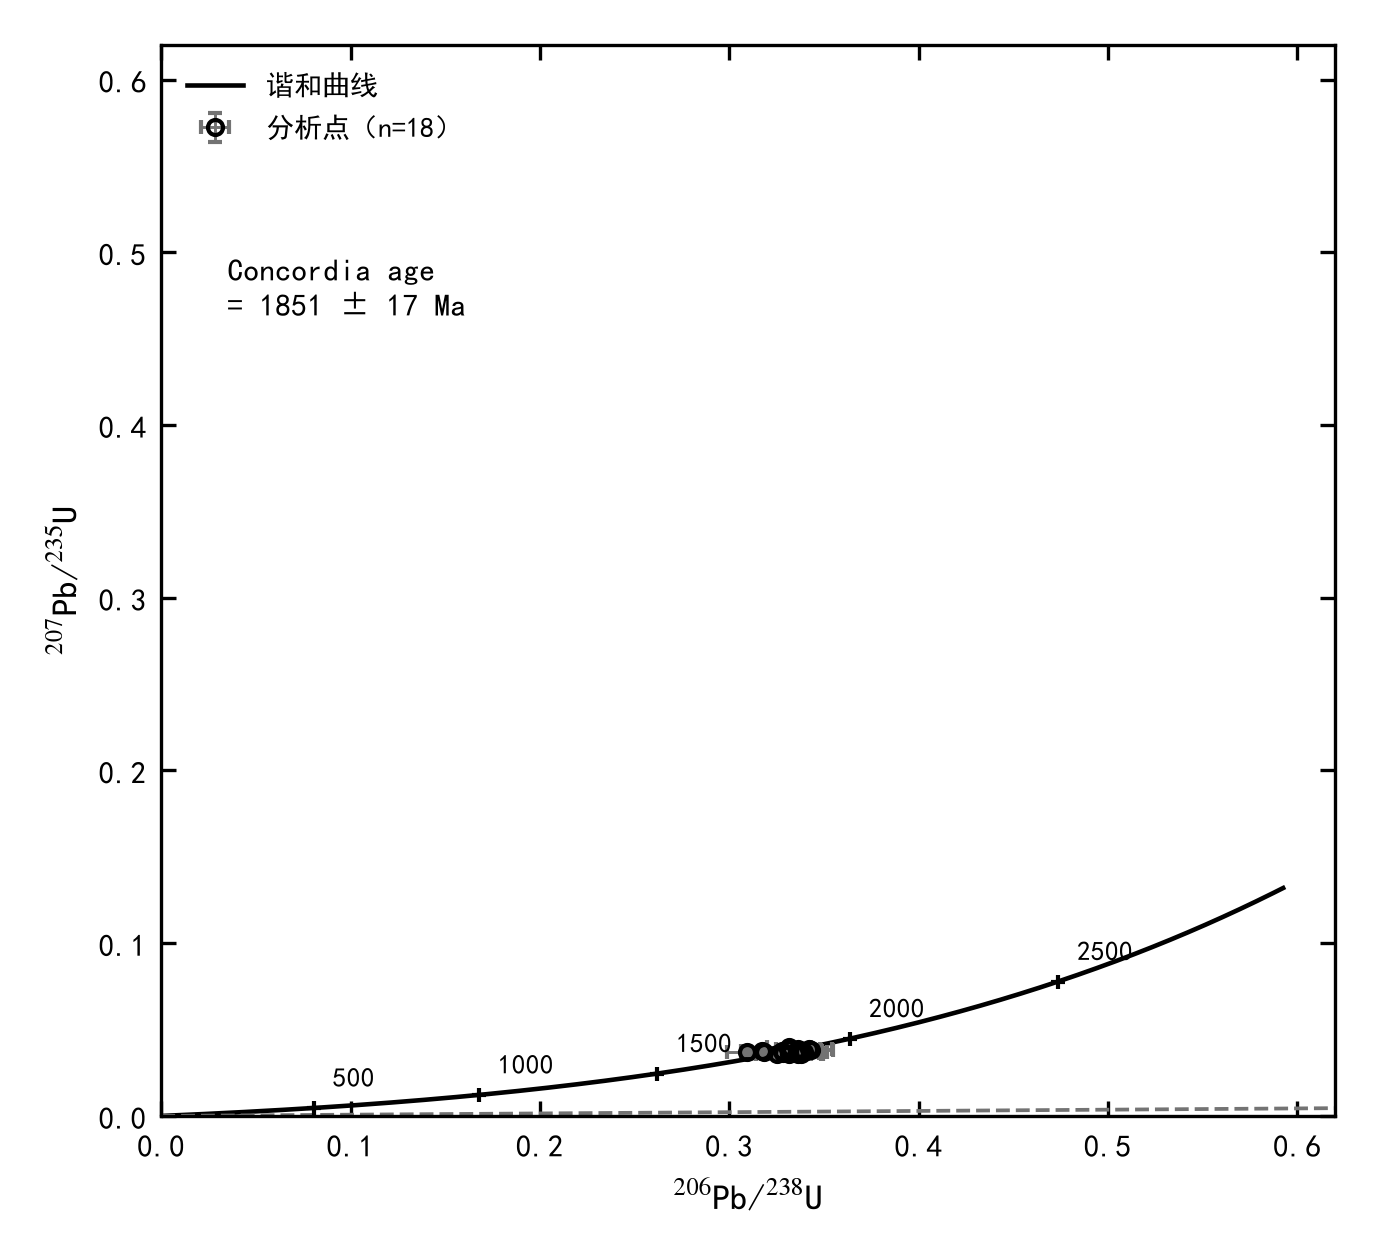
\includegraphics[width=.58\textwidth]{figs/fig_uPb_concordia.png}
    \caption{锆石 U-Pb 谐和图}
    \label{fig:concordia}
\end{figure}

\section{全岩主量元素}

主量元素分析结果列于表 \ref{tab:major}。岩石
$\mathrm{SiO_2}$ 含量为 $63.2\%\sim68.7\%$，
$\mathrm{Al_2O_3}$ 为 $14.6\%\sim16.2\%$，
全碱含量 $\mathrm{K_2O}+\mathrm{Na_2O}=6.1\%\sim7.4\%$，
$\mathrm{K_2O/Na_2O}=1.02\sim1.38$，属高钾钙碱性系列。
铝饱和指数 A/CNK 为 $0.96\sim1.05$，为准铝质—弱过铝质岩石。

\begin{table}[htbp]
    \centering
    \caption{代表性样品主量元素含量（$w_\mathrm{B}$/\%）}
    \label{tab:major}
    \small
    \begin{tabular}{lcccccc}
        \toprule
        组分 & S-1 & S-2 & S-3 & S-4 & S-5 & S-6 \\
        \midrule
        $\mathrm{SiO_2}$ & 65.3 & 68.7 & 63.2 & 66.1 & 67.4 & 64.8 \\
        $\mathrm{TiO_2}$ & 0.58 & 0.42 & 0.71 & 0.55 & 0.47 & 0.62 \\
        $\mathrm{Al_2O_3}$ & 15.4 & 14.6 & 16.2 & 15.1 & 14.9 & 15.8 \\
        $\mathrm{Fe_2O_3^T}$ & 4.21 & 3.12 & 5.08 & 4.02 & 3.55 & 4.46 \\
        $\mathrm{MgO}$ & 2.14 & 1.52 & 2.86 & 2.03 & 1.74 & 2.31 \\
        $\mathrm{CaO}$ & 3.52 & 2.61 & 4.18 & 3.36 & 2.94 & 3.71 \\
        $\mathrm{Na_2O}$ & 3.41 & 3.02 & 3.66 & 3.28 & 3.15 & 3.52 \\
        $\mathrm{K_2O}$ & 3.48 & 4.11 & 2.61 & 3.72 & 4.05 & 3.12 \\
        $\mathrm{P_2O_5}$ & 0.16 & 0.11 & 0.21 & 0.15 & 0.13 & 0.18 \\
        \midrule
        A/CNK & 0.98 & 1.02 & 0.96 & 1.00 & 1.05 & 0.99 \\
        \bottomrule
    \end{tabular}
\end{table}

\section{微量元素与稀土元素}

稀土元素总量 $\Sigma\mathrm{REE}$ 为 $128\times10^{-6}\sim214\times10^{-6}$，
轻重稀土分异明显，$(\mathrm{La/Yb})_\mathrm{N}=8.6\sim14.2$，
$\delta\mathrm{Eu}$ 为 $0.52\sim0.78$，显示中等负铕异常
（图 \ref{fig:ree}）。微量元素蛛网图表现为大离子亲石元素
（Rb、Ba、Th、U）富集，高场强元素（Nb、Ta、Ti）明显亏损，
与俯冲带岩浆岩的典型特征一致。

\begin{figure}[htbp]
    \centering
    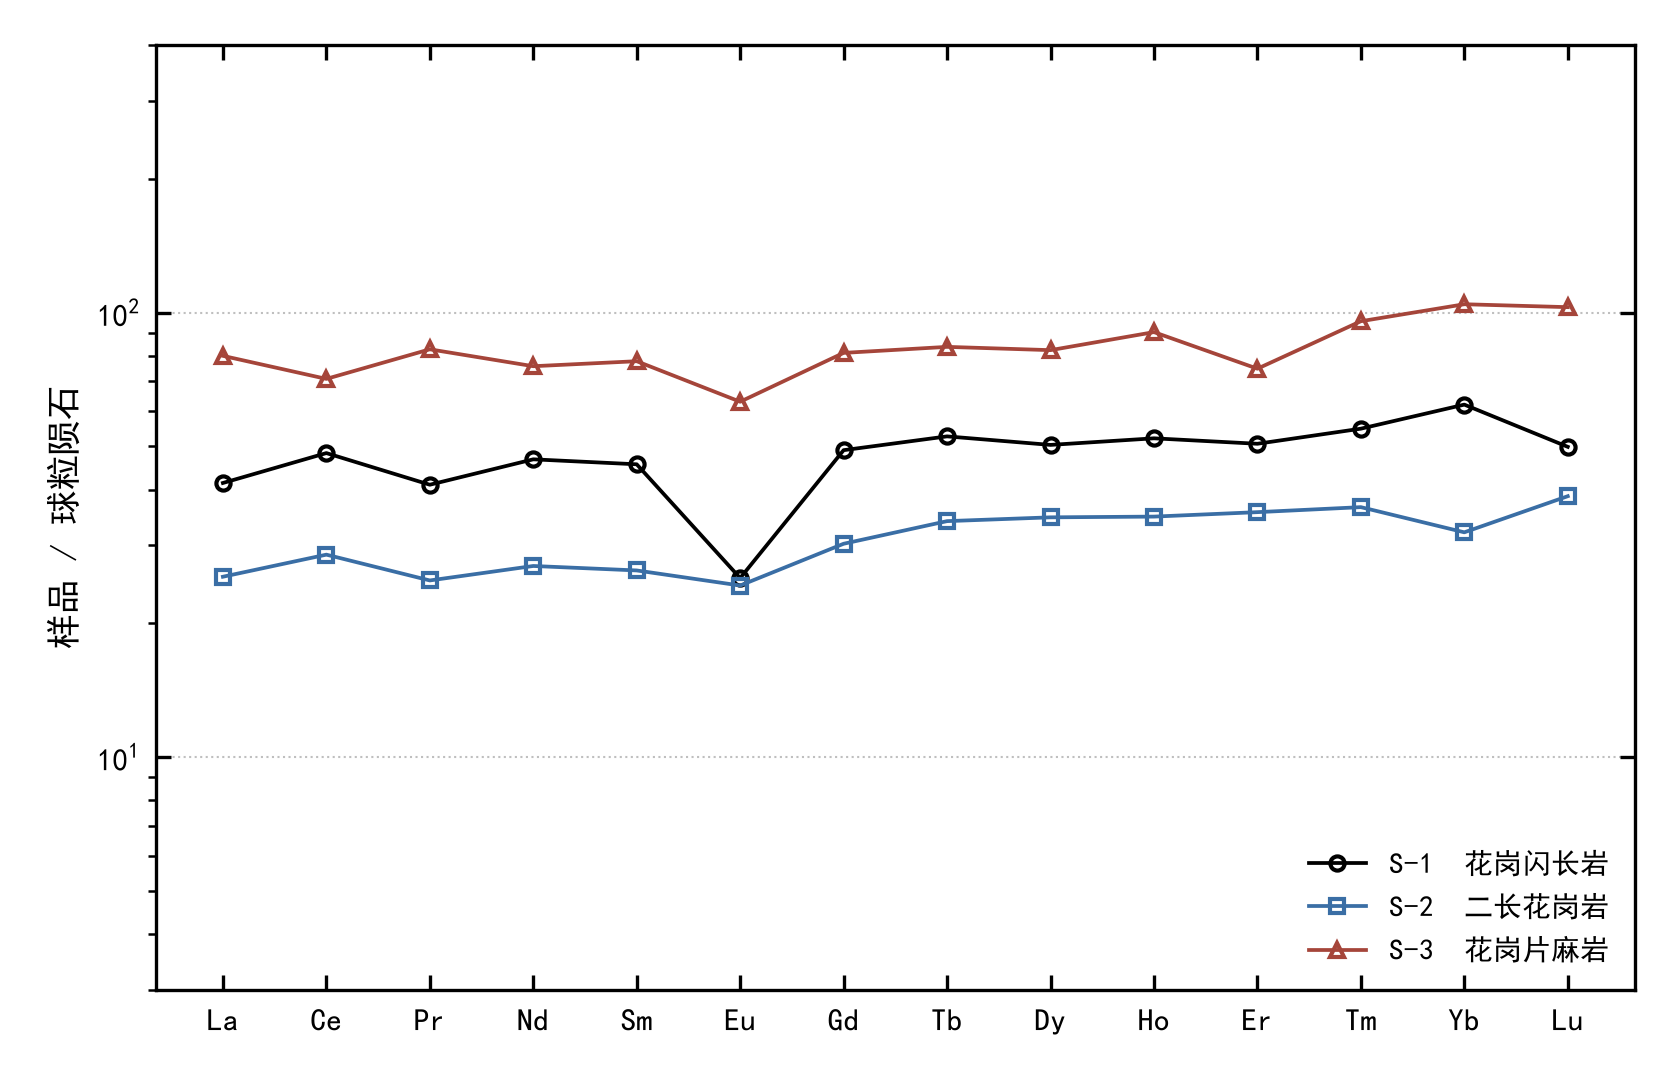
\includegraphics[width=.78\textwidth]{figs/fig_ree_pattern.png}
    \caption{花岗岩稀土元素球粒陨石标准化配分模式图
        （标准化值据 Boynton，1984）}
    \label{fig:ree}
\end{figure}

% =============================================================
\chapter{讨论}

\section{岩石成因}

岩石具有较高的 $\mathrm{SiO_2}$ 与全碱含量、较低的 Mg\#
（$38\sim46$），且富集 LILE、亏损 HFSE，
表明其源区以壳源物质为主，同时有幔源组分的参与。
中等负 Eu 异常说明岩浆经历了斜长石的分离结晶，
或源区存在斜长石的残留。

结合区域上同期基性—超基性岩的发育，推测幔源岩浆的底侵
为下地壳部分熔融提供了热源，形成本文所研究的花岗质岩石。

\section{构造意义}

综合年代学与地球化学证据，本文认为该期岩浆活动形成于
活动大陆边缘的俯冲背景，与古特提斯洋向北的俯冲消减有关。
该年龄的确定为约束东昆仑地区晚古生代构造演化时限
提供了新的资料。

% =============================================================
\chapter{结论}

本文对东昆仑造山带中段晚古生代花岗岩体开展了系统的年代学与
地球化学研究，获得以下主要认识：

\begin{enumerate}
    \item 锆石 LA-ICP-MS U-Pb 定年获得 $1851\pm17$ Ma 的加权平均年龄，
        代表岩体的侵位时代；
    \item 岩石属高钾钙碱性、准铝质—弱过铝质系列，
        富集大离子亲石元素、亏损高场强元素，具中等负 Eu 异常；
    \item 岩石成因以壳源物质部分熔融为主，幔源岩浆底侵提供了热源，
        形成于活动大陆边缘的俯冲背景。
\end{enumerate}

% =============================================================
\backmatter
% 规范 1.13 / 1.14 / 1.15 的顺序：参考文献 -> 致谢 -> 附录
% BibTeX 条目类型：期刊论文 article、专著 book、编著章节 incollection、
% 学位论文 phdthesis / mastersthesis、会议论文 inproceedings、标准 standard。
% 注意 BibTeX 不认百分号注释，.bib 条目区里不要出现 at 符号。
\cugthesisbib{sample}
\cugthesisacknowledgements

\appendix
\chapter{附录 A\quad 分析测试数据}

\begin{table}[htbp]
    \centering
    \caption{锆石微量元素分析结果（$w_\mathrm{B}$/$10^{-6}$）}
    \label{tab:appendix}
    \small
    \begin{tabular}{lcccccc}
        \toprule
        元素 & 01 & 02 & 03 & 04 & 05 & 06 \\
        \midrule
        Ti  & 12.4 & 9.8  & 14.1 & 11.2 & 10.5 & 13.3 \\
        Y   & 842  & 761  & 918  & 806  & 779  & 887  \\
        Nb  & 3.12 & 2.68 & 3.54 & 2.97 & 2.81 & 3.36 \\
        Hf  & 9124 & 8862 & 9451 & 9028 & 8917 & 9306 \\
        Th  & 186  & 152  & 214  & 173  & 161  & 198  \\
        U   & 312  & 268  & 351  & 296  & 281  & 331  \\
        \bottomrule
    \end{tabular}
\end{table}

\end{document}
